\chapter{相关技术背景}
本章主要包含三个部分:
1.首先对Top-k算法原理进行了详细的介绍,引出了RadixSelect算法并阐述了选择它进行实现的理由。
2.介绍了国产AI处理器的编程模型和内存模型。
3.为方便后续验证Top-k算子的可用性,介绍了面向国产AI处理器的pytorch框架。
\section{Top-k算法原理}

如前文所述,在并行Top-k算法领域,已有诸多值得关注的研究成果。在众多成果当中,基于选择的
并行Top-k算法相较于全排序算法具有明显的领先优势。
基于选择的并行Top-K算法包括
QuickSelect、BucketSelect 、RadixSelect 以及SampleSelect\cite{alabi2012fast}\cite{ribizel2020parallel}。
其中QuickSelect以快速排序为基础,然而其与传统排序算法的差异在于,
它仅在包含第$K$个元素的子列表上展开迭代操作。此过程通过递归方式持续进行,
直至所选枢轴最终确定为第$K$个元素,并且在前$K$个元素的确定过程中,通过递归收集
逐步达成目标。BucketSelect、SampleSelect和RadixSelect则采用多个枢轴,将候
选元素分配至数十到数百个桶中。BucketSelect的枢轴确定依赖于候选元素的最小值与最
大值;SampleSelect通过对一小部分元素进行采样并排序,以获取更为适宜的枢轴;
RadixSelect与最高有效位基数排序相似,依据元素的数位特征将元素分配至相应桶中。
而相较于其他三种基于选择的方法,RadixSelect具备若干显著优势:

\begin{enumerate}
\item 在最坏情况下,其时间复杂度为$O(N)$。假设在RadixSelect算法中,一个$r$位数字被分
割为$b$位数字,那么最多仅需$\left\lceil\frac{r}{b}\right\rceil$次迭代。
因此,无论是平均情况还是最坏情况,其时间复杂度均为
$O(\left\lceil\frac{r}{b}\right\rceil N)$。
相比之下,QuickSelect算法在最坏情形下,每次迭代仅能移除一个元素。由此,
处理大约$N$个元素时,$N$次迭代将导致其最坏情况时间复杂度达到$O(N^{2})$。

\item 在GPU上,当采用8位或11位数字(分别对应256个或2048个桶)时,RadixSelect能展现出高度的
并行性,能够更为有效地削减计算工作量。

\item BucketSelect和SampleSelect在选择枢轴时均需计算输入数据的统计信息,而RadixSelect的枢轴选择与输入数据相互独立\cite{zhang2023parallel}。

\end{enumerate}
基于以上原因,本文主要基于RadixSelect算法对Top-k算子进行并行实现。
RadixSelect算法基于基数排序思想,用于在无序数组中找到第k小(或大)的元素,
首先将元素的二进制表示按每连续b位划分为一个数位(digit),从最高有效位开始处理,
每次迭代处理一个数位。对于r位元素,共需$\left\lceil\frac{r}{b}\right\rceil$次迭代。
而对于每次迭代,其核心步骤如下:
\begin{enumerate}
    
    \item  {计算直方图}:在每次迭代中,提取每个元素当前处理数位的b位并转换为对应的digit值(范围是$[0, 2^{b}-1]$),然后计算直方图以记录每个digit值出现的频率,即直方图的第i个计数器记录digit值等于i的元素数量。
    \item  {计算前缀和}:对直方图计算前缀和(inclusive prefix sum),得到前缀和数组psum。(psum[i]表示digit值小于或等于i的元素数量)。
    \item  {确定目标数位}:通过前缀和数组找到第k小元素应具有的digit值j,满足psum[j - 1] < K且psum[j] ≥ K。
    \item  {筛选元素}:将digit值小于j的元素确定为当前的Top - k元素,存储其值和索引;digit值大于j的元素可直接丢弃;digit值等于j的元素作为潜在结果存储到候选缓冲区,用于下一次迭代。
    \item  {更新参数}:每次迭代结束后,更新k(减去已确定的Top - k元素数量psum[j - 1])和n(更新为直方图中digit值等于j的元素数量),为下一次迭代做准备。
\end{enumerate}
在算法执行过程中,通过不断迭代上述步骤,逐步缩小候选元素范围,直到找到第k小(或大)的元素。
为了更好的说明上述步骤,下图~\ref{fig:radixselect}介绍了如何从9个元素当中获取Top-4个元素。

\begin{figure}[ht]
    \centering
    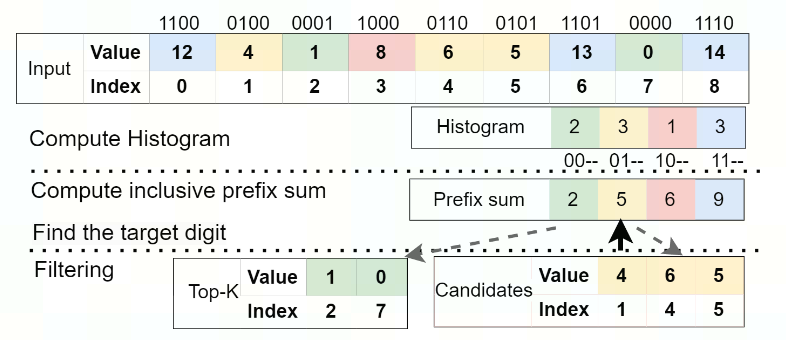
\includegraphics[width=1.0\textwidth]{radixselect.png}
    \caption{RadixSelect流程图}
    \label{fig:radixselect}
    % \note{注:图注的内容不宜放到图题中。}
\end{figure}

对于9个4位元素的列表(以2位为一个数位),第一次迭代计算最高2位的直方图,而后
根据直方图信息计算出前缀和,
再根据第k小元素(k = 4)的条件确定目标数位为'01',此时digit值为'00'的元素成为部分结果,
digit值为'01'的元素进入候选缓冲区用于下一次迭代,同时更新k和n,继续后续迭代直至找到最终的Top - k元素。




\section{国产AI处理器概述}
本文基于寒武纪多核深度学习处理器(Deep Learning Processor-Multicore,DLP-M)
实现Top-k算子,下面主要从体系结构,内存层次,编程模型三个方面对其进行介绍。
\subsection{抽象硬件模型}
DLP-M硬件的基本组成单元是MLU Core。每个 MLU Core 是具备完整计算、IO和控制功能的处理器核心,可以独立完成一个计算任务,
也可以与其他 MLU Core 协作完成一个计算任务。每4个 MLU Core 核心构成一个 Cluster,另外,其每个 Cluster 内还会包含一个
额外的 Memory Core 和一块被 Memory Core 和 4 个 MLU Core 共享的 SRAM(Shared RAM,共享存储单元)。
Memory Core 不能执行向量和张量计算指令,只能用于 SRAM 与 DDR (Double Data Rate Synchronous Dynamic Random Access Memory,
双倍速率同步动态随机存储器,DDR SDRAM通常简称为DDR) 和 MLU Core 之间的数据传输。
Cambricon BANG 异构并行计算平台对底层由 MLU 硬件构成的大规模并行计算系统进行了一系列抽象,屏蔽了具体硬件之间的细微差异,
向用户展示了一个高度并行、灵活扩展和易于操控的抽象硬件模型。Cambricon BANG异构并行编程模型由通用处理器和多个 MLU 领域专用处理器组成。
其中,MLU 负责核心的大规模并行计算,而通用处理器则作为控制单元,负责复杂控制和任务调度等工作
。整个抽象硬件模型分为5个层级:服务器级、板卡级、芯片级、处理器簇(Cluster)级和 MLU Core 级,
每个层次都包括抽象的控制单元、计算单元和存储单元,
如图~\ref{fig:arch}所示。
\begin{figure}[ht]
    \centering
    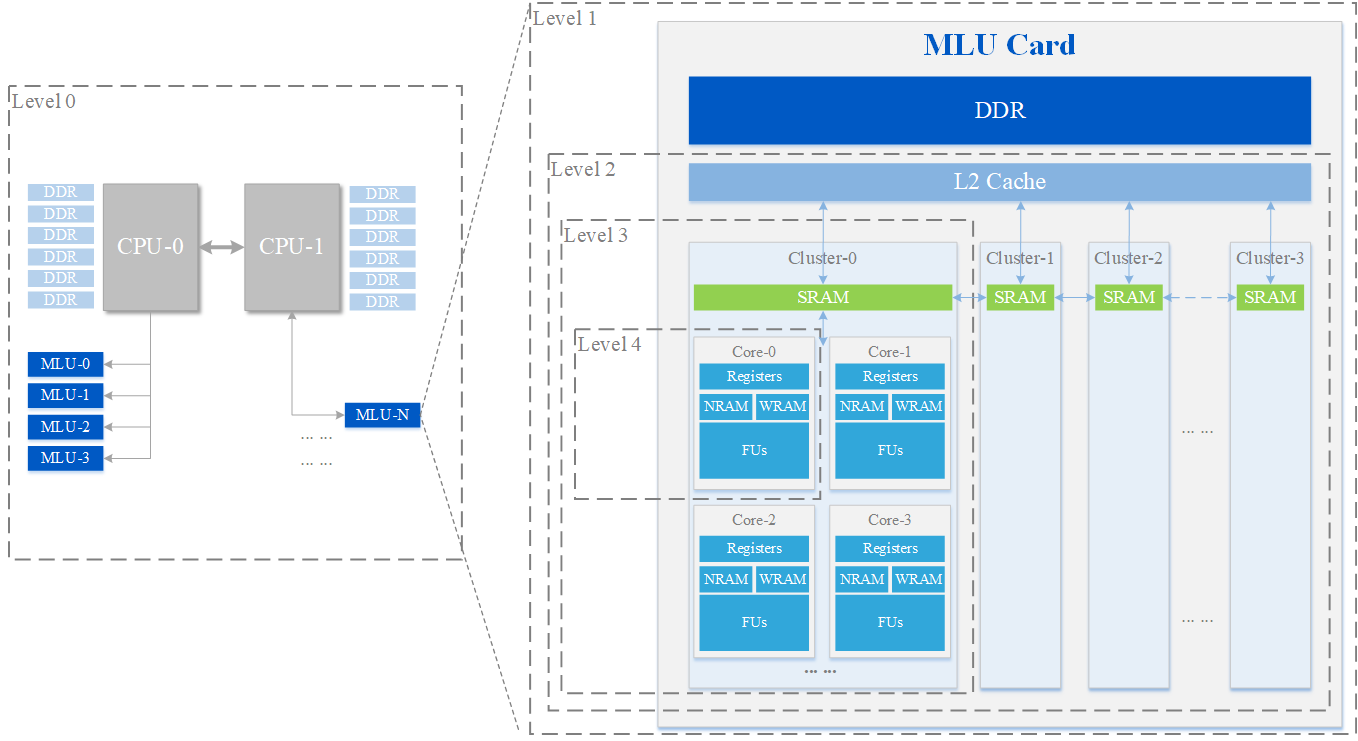
\includegraphics[width=0.8\textwidth]{arch.png}
    \caption{DLP-M 架构图}
    \label{fig:arch}
    \note{}
  \end{figure}

\begin{enumerate}

\item 第0级是服务器级,由多个 CPU 构成的控制单元、本地 DDR 存储单元和多个 MLU 板卡构成的计算单元组成;

\item 第1级是板卡级,每个 MLU 板卡由本地控制单元、DDR 存储单元和 MLU 芯片构成的计算单元组成;

\item 第2级是芯片级,每个芯片由本地控制单元、本地存储单元(例如 L2 Cache)以及一个或者多个 Cluster 构成的计算单元组成;

\item 第3级是 Cluster 级,每个 Cluster 由本地控制单元、共享存储以及多个 MLU Core 构成的计算单元组成;

\item 第4级是 MLU Core 级,每个 MLU Core 由本地控制单元、私有存储单元和计算单元组成。在 MLU Core 内部支持指令级并行和数据级并行。
\end{enumerate}
整个抽象硬件模型可以通过增加服务器数量、板卡数量、芯片数量、Cluster 数量或者 MLU Core 数量的方式自由扩展计算能力。
本文的主要内容为算子开发工作,主要涉及到1-4级。

\subsection{内存模型}
抽象硬件模型提供了丰富的存储层次,包括GPR(General Purpose Register,通用寄存器)、NRAM、WRAM、SRAM、L2 Cache、LDRAM(Local DRAM,局部 DRAM 存储单元)、
GDRAM(Global DRAM,全局 DRAM 存储空间)等。GPR、WRAM 和 NRAM 是一个 MLU Core 的私有存储,Memory Core 没有私有的 WRAM 和 NRAM 存储资源。
L2 Cache 是芯片的全局共享存储资源,目前主要用于缓存指令、Kernel 参数以及只读数据。LDRAM 是每个 MLU Core 和 Memory Core 的私有存储空间,
其容量比 WRAM 和 NRAM 更大,主要用于解决片上存储空间不足的问题。GDRAM 是全局共享的存储资源,可以用于实现主机端与设备端的数据共享,以及计算任务之间的数据共享。
抽象的硬件模型允许软件直接控制数据在各级存储之间的移动,从而高效地完成计算任务。为此,编译器对上层软件提供了丰富的地址空间声明,以及大量用于显式或隐式数据移动的
机制和编程接口,以方便用户显式控制数据的存储空间。用户可以显式地控制数据在各个存储层次之间的移动,精确地控制数据搬运的时机和数据量,从而实现计算和 IO 之间的平衡,
最大化计算效率。其内存层次图如图~\ref{fig:memory}所示
\begin{figure}[ht]
    \centering
    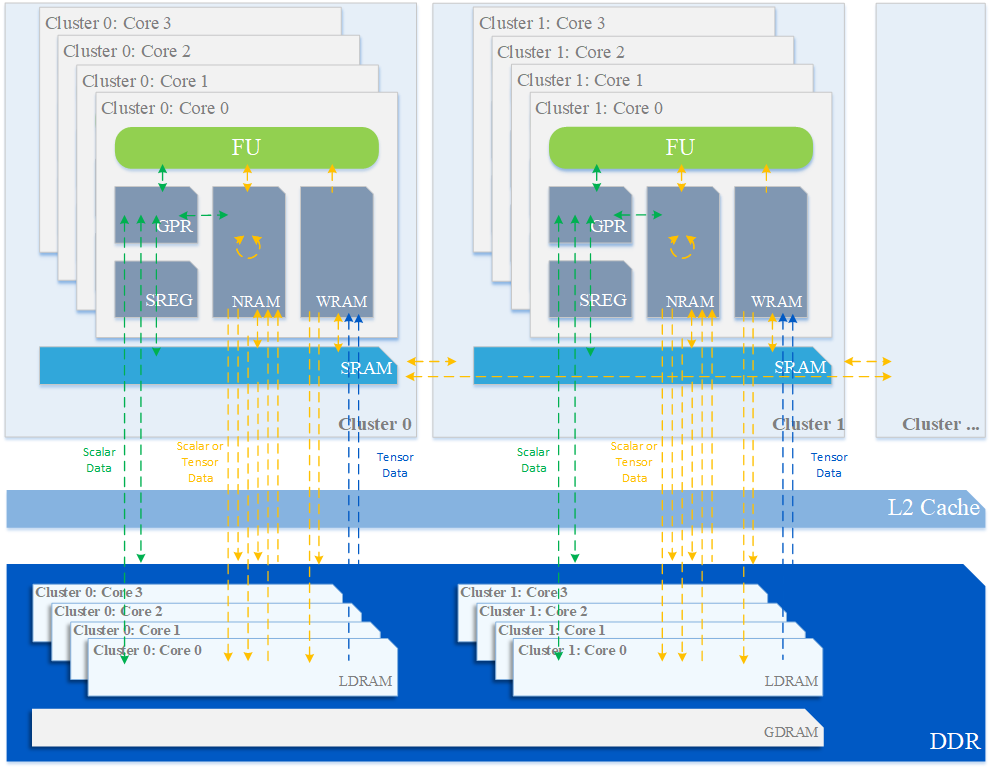
\includegraphics[width=0.8\textwidth]{memory.png}
    \caption{内存层次图}
    \label{fig:memory}
    \note{}
  \end{figure}

  \begin{enumerate}
  \item GPR 是每个 MLU Core 和 Memory Core 私有的存储资源。MLU Core 和 Memory Core 的标量计算系统都采用精简指令集架构,所有的标量数据,无论是整型数据还是浮点数据,在参与运算之前必须先加载到 GPR。GPR 的最大位宽为 48位,一个GPR 可以存储一个 8bit、16bit、32bit或者48bit的数据。GPR 中的数据不仅可以用来实现标量运算和控制流功能,还用于存储向量运算所需要的地址、长度和标量参数等。
  \item NRAM 是每个 MLU Core 私有的片上存储空间,主要用来存放向量运算和张量运算的输入和输出数据,也可以用于存储一些运算过程中的临时标量数据。相比 GDRAM 和 LDRAM 等片外存储空间,NRAM 有较低的访问延迟和更高的访问带宽。NRAM 的访存效率比较高但空间大小有限,而且不同硬件的 NRAM 容量不同。用户需要合理利用有限的 NRAM 存储空间,以提高程序的性能。对于频繁访问的数据,应该尽量放在 NRAM 上,仅仅当 NRAM 容量不足时,才将数据临时存储在片上的 SRAM 或者片外的 LDRAM 或者 GDRAM 上。
  \item WRAM 是每个 MLU Core 私有的片上存储空间,主要用来存放卷积运算的卷积核数据。为了高效地实现卷积运算,
  WRAM 上的数据具有特殊的数据布局
  \item SRAM 是一个 Cluster 内所有 MLU Core 和 Memory Core 都可以访问的共享存储空间。SRAM 可以用于缓存 MLU Core 的中间计算结果,实现 Cluster 内不同 MLU Core 或 Memory Core 之间的数据共享及不同 Cluster 之间的数据交互。SRAM 有较高的访存带宽,但是容量有限。用户需要合理利用有限的 SRAM 存储空间,以提高程序的性能。
  \item L2 Cache 是位于片上的全局存储空间,由硬件保证一致性,目前主要用于缓存指令、Kernel 参数以及只读数据。L2 Cache 目前对于用户透明,在 Cambricon BANG 异构并行编程模型中暂时没有提供读写 L2 Cache 的接口。
  \item LDRAM 是每个 MLU Core 和 Memory Core 私有的存储空间,可以用于存储无法在片上存放的私有数据。LDRAM 属于片外存储,不同 MLU Core 和 Memory Core 之间的LDRAM空间互相隔离,软件可以配置其容量。与GDRAM相比,LDRAM的访存性能更好,因为LDRAM的访存冲突比较少。
  \item 与 LDRAM 类似,GDRAM 也是片外存储。位于 GDRAM 中的数据被所有的 MLU Core 和 Memory Core 共享。GDRAM 空间的作用之一是用来在主机侧与设备侧传递数据,如 Kernel 的输入、输出数据等。Cambricon BANG 异构编程模型提供了专门用于在主机侧和设备侧之间进行数据拷贝的接口。
\end{enumerate}
\subsection{编程模型}
国产AI处理器的异构并行编程模型利用CPU和MLU协同计算,实现了CPU和MLU的优势互补。
在并行编程模型中,CPU 作为主机侧的控制设备,用于完成复杂的控制和任务调度;
而设备侧的 MLU 则用于大规模并行计算和领域相关的计算任务。
执行的程序称作Kernel函数(核函数),在核函数被执行之前,往往需要根据任务规模来决定需要多少个Job进行处理。

在MLU上被调度的最小单位被称为Job(作业),其被调度到Cluster执行(需要满足一定的规则才可以被调度),
Job之间一般也是逻辑独立的。一个Job至少包含一个Task,具体视类型而定。
因此被执行的最小单位为Task(任务),其被调度到具体的MLU-Core上执行,执行一遍核函数中的程序代码。

而Job又可以分为不同的类型,其代表着此Job所需要的硬件资源数量,
即一个Job在实际执行时会启动多少个物理 MLU Core 或者 Cluster。
在其并行编程模型中支持两种任务类型:Block 类型和 UnionX 类型。
\begin{enumerate}

    \item{Block}:代表一个Job在执行时至少需要占用一个 MLU Core。对于 Block 类型的Job,
    不支持共享 SRAM,不支持不同 Cluster 之间的通信。Block类型的Job是所有MLU-Core硬件都支持的类型。
    当Job规模大于1时,由计算平台根据硬件资源占用情况决定所有Job占用的 MLU Core 数量:
    如果只有一个 MLU Core 可用,那么所有Job在同一个 MLU Core 上串行执行;
    如果有多个物理 MLU Core 可用,那么所有Job会被平均分配到所有可用的 MLU Core 上分批次执行。
    \item {UnionX}:表示一个 Job 在执行时至少需要占用 X 个 Cluster,其中,X 必须为2的整数次幂。
    一个拥有 M 个 Cluster 的板卡,X的最大值为 \(2\lfloor\log_2 M\rfloor\)。

    MLU-Core 对 Union 类型Job的支持与硬件的具体配置有关。例如,一些终端侧或者边缘侧的单核设备不支持 
    Union类型,而一个拥有8个 Cluster 的硬件只能够支持 Union1、Union2、Union4 和 Union8 类型的 Job,
    无法支持 Union16 类型的Job。
    

\end{enumerate}



\section{面向深度学习的处理器的pytorch框架}

为支持国产AI处理器,寒武纪定制了开源人工智能编程框架PyTorch(以下简称Cambricon PyTorch)。
Cambricon PyTorch借助PyTorch自身提供的设备扩展接口将MLU后端库中所包含的算子操作动态注册到PyTorch中,MLU后端库可处理MLU上的张量和算子的运算。Cambricon PyTorch会基于Cambricon CNNL库在MLU后端实现一些常用算子,并完成一些数据拷贝。
为了能在Torch模块方便使用MLU设备,Cambricon PyTorch在PyTorch后端进行了以下扩展:
\begin{enumerate} 
\item 通过Torch模块可调用MLU后端支持的网络运算。

\item 对MLU暂不支持的算子,支持该类算子自动切换到CPU上运行。

\item Torch模块中与MLU相关的接口的语义与CPU和GPU的接口语义保持一致。
\end{enumerate}
为便于进行PyTorch和基于深度学习处理器的Top-k实现关系的理解,此处对国产AI处理器的整体软件栈结构进行介绍。
在其软件栈中,如下图\ref{fig:level}所示。
PyTorch等通过调用Cambricon CNNL算子接口,
实现对应的框架层算子在MLU上的高性能加速计算。而Cambricon CNNL作为一个网络运算库,提供了人工智能计算所需要
的算子接口。Cambricon CNNL算子的计算通过软件栈底层CNRT(Cambricon Runtime Library,寒武纪运行时库
)和CNDrv 接口(Cambricon Driver API,寒武纪驱动API)完成与寒武纪MLU设备底层驱动的交互和计算任务。


\begin{figure}[ht]
    \centering
    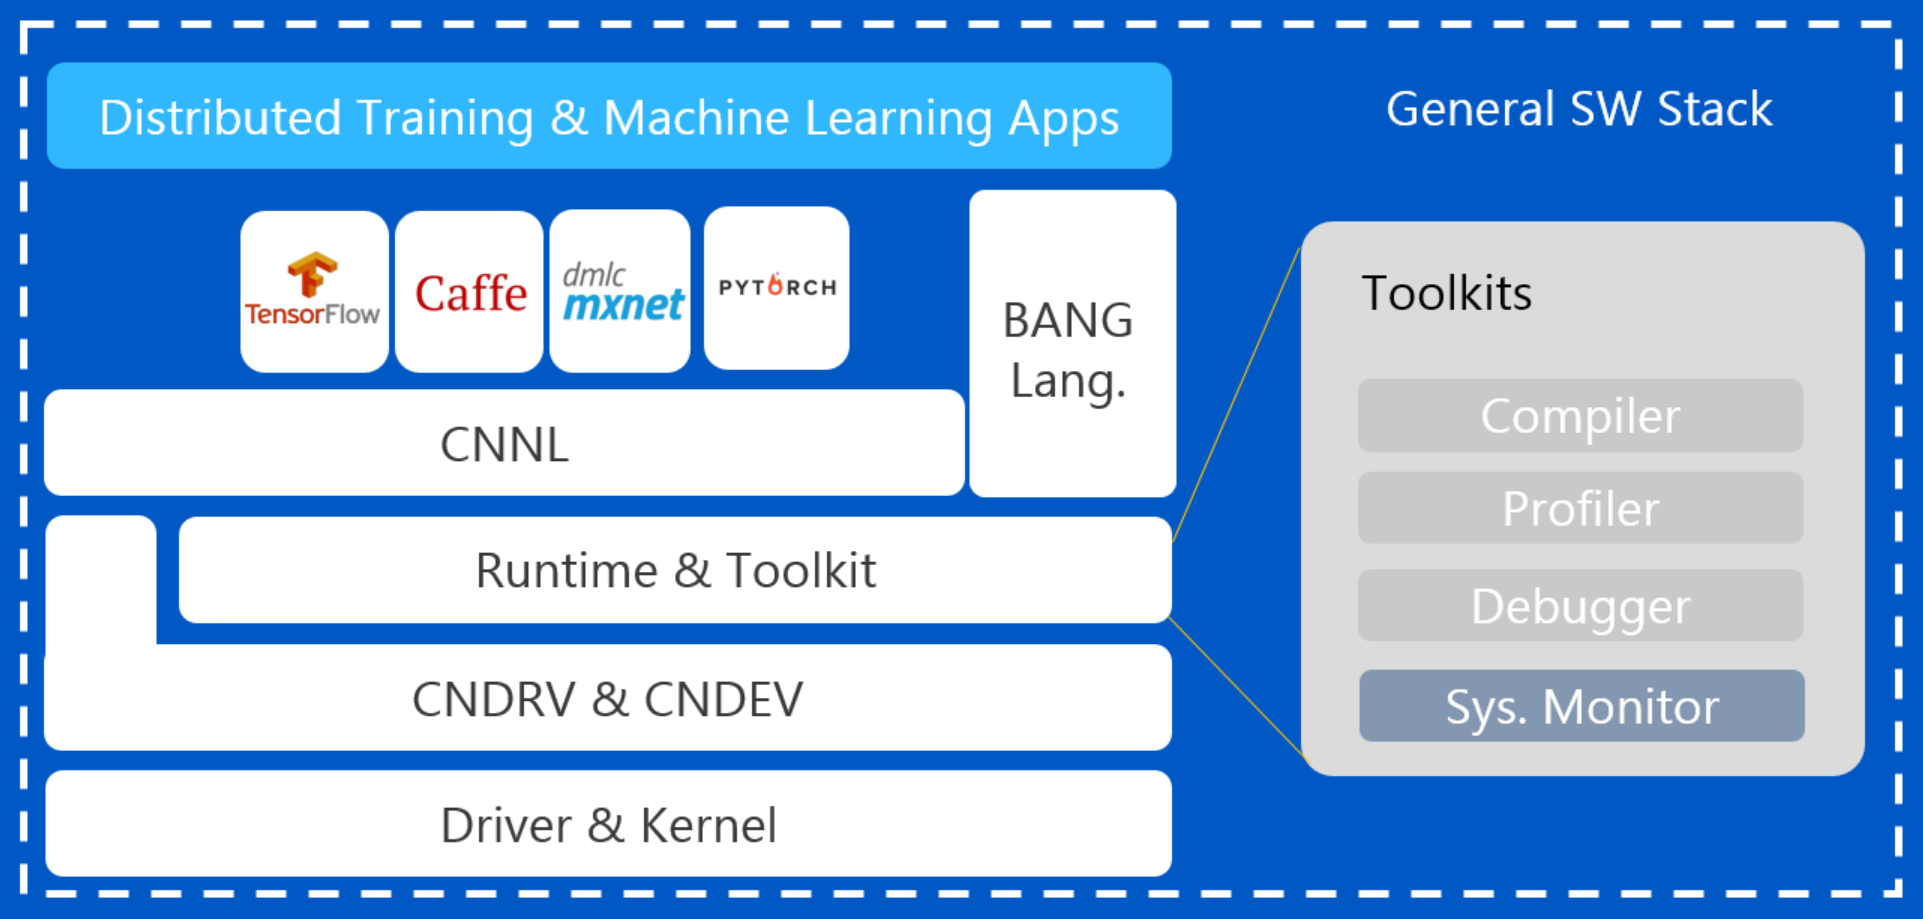
\includegraphics[width=1.0\textwidth]{level.png}
    \caption{软件栈示意图}
    \label{fig:level}
    \note{}
  \end{figure}



\section{本章小结}
本章首先详细阐述了RadixSelect算法的基本原理,为后续在国产AI处理器上实现高效的Top-k算子奠定了理论基础。
随后,深入介绍了国产AI处理器的硬件架构,并从抽象硬件模型,内存模型和编程模型三个层面,
详尽地介绍了基于国产AI处理器的异构计算平台,为后续如何对Top-k算子进行实现和性能优化指明了方向。
最后介绍了面向国产AI处理器的Pytorch框架,为后续验证Top-k算子可用性提供了方案参考。